


\tikzset{every picture/.style={line width=0.75pt}} %set default line width to 0.75pt        

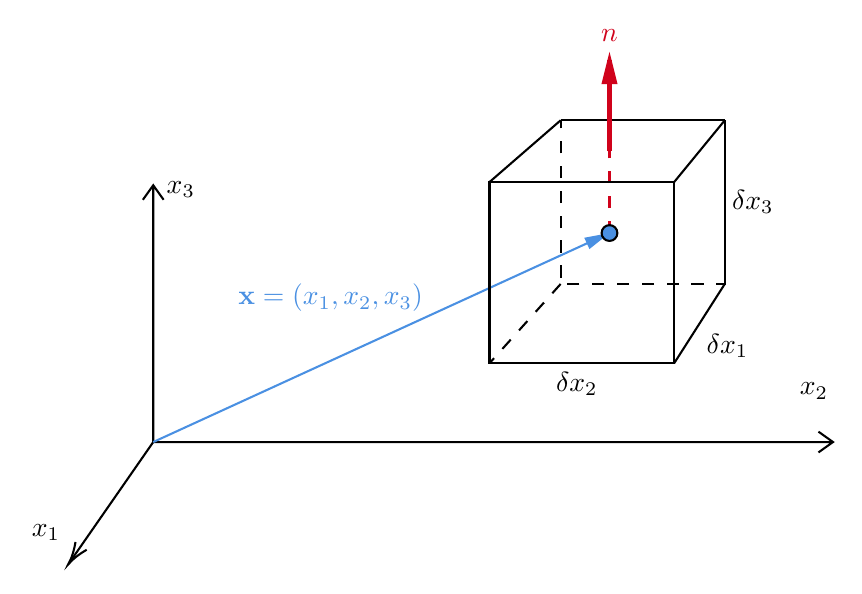
\begin{tikzpicture}[x=0.75pt,y=0.75pt,yscale=-1,xscale=1]
%uncomment if require: \path (0,280); %set diagram left start at 0, and has height of 280

%Shape: Axis 2D [id:dp5518401001098778] 
\draw  (121,213) -- (448.5,213)(121,89.28) -- (121,213) -- cycle (441.5,208) -- (448.5,213) -- (441.5,218) (116,96.28) -- (121,89.28) -- (126,96.28)  ;
%Straight Lines [id:da26796887697132976] 
\draw    (121,213) -- (81.14,270.36) ;
\draw [shift={(80,272)}, rotate = 304.8] [color={rgb, 255:red, 0; green, 0; blue, 0 }  ][line width=0.75]    (10.93,-3.29) .. controls (6.95,-1.4) and (3.31,-0.3) .. (0,0) .. controls (3.31,0.3) and (6.95,1.4) .. (10.93,3.29)   ;
%Straight Lines [id:da11690039881602576] 
\draw    (371.97,175.05) -- (396.35,136.86) ;
%Straight Lines [id:da1387258518267478] 
\draw    (396.35,136.86) -- (396.35,58) ;
%Straight Lines [id:da12411065407885058] 
\draw    (371.97,87.74) -- (396.35,58) ;
%Straight Lines [id:da6511153232143523] 
\draw    (283,87.74) -- (317.27,58) ;
%Straight Lines [id:da5071674849590391] 
\draw    (317.27,58) -- (396.35,58) ;
%Shape: Rectangle [id:dp9982277363088392] 
\draw  [dash pattern={on 4.5pt off 4.5pt}] (317.27,58) -- (396.35,58) -- (396.35,136.86) -- (317.27,136.86) -- cycle ;
%Straight Lines [id:da9554819819366029] 
\draw  [dash pattern={on 4.5pt off 4.5pt}]  (317.27,136.86) -- (283,175.05) ;
%Straight Lines [id:da9451944557846346] 
\draw [color={rgb, 255:red, 208; green, 2; blue, 27 }  ,draw opacity=1 ] [dash pattern={on 4.5pt off 4.5pt}]  (340.82,112.3) -- (340.82,73) ;
%Straight Lines [id:da9452427593542412] 
\draw [color={rgb, 255:red, 208; green, 2; blue, 27 }  ,draw opacity=1 ][line width=1.5]    (340.82,73) -- (340.82,29) ;
\draw [shift={(340.82,25)}, rotate = 90] [fill={rgb, 255:red, 208; green, 2; blue, 27 }  ,fill opacity=1 ][line width=0.08]  [draw opacity=0] (15.6,-3.9) -- (0,0) -- (15.6,3.9) -- cycle    ;
%Straight Lines [id:da5417958009997437] 
\draw [color={rgb, 255:red, 74; green, 144; blue, 226 }  ,draw opacity=1 ]   (121,213) -- (339,113.13) ;
\draw [shift={(340.82,112.3)}, rotate = 155.39] [fill={rgb, 255:red, 74; green, 144; blue, 226 }  ,fill opacity=1 ][line width=0.08]  [draw opacity=0] (12,-3) -- (0,0) -- (12,3) -- cycle    ;
%Shape: Rectangle [id:dp9250778191688305] 
\draw  [color={rgb, 255:red, 0; green, 0; blue, 0 }  ,draw opacity=1 ] (283,87.74) -- (371.97,87.74) -- (371.97,175.05) -- (283,175.05) -- cycle ;
%Shape: Ellipse [id:dp48060961846918415] 
\draw  [fill={rgb, 255:red, 74; green, 144; blue, 226 }  ,fill opacity=1 ] (337.02,112.3) .. controls (337.02,110.2) and (338.72,108.5) .. (340.82,108.5) .. controls (342.92,108.5) and (344.62,110.2) .. (344.62,112.3) .. controls (344.62,114.4) and (342.92,116.1) .. (340.82,116.1) .. controls (338.72,116.1) and (337.02,114.4) .. (337.02,112.3) -- cycle ;

% Text Node
\draw (61,251.4) node [anchor=north west][inner sep=0.75pt]    {$x_{1}$};
% Text Node
\draw (431,183.03) node [anchor=north west][inner sep=0.75pt]    {$x_{2}$};
% Text Node
\draw (126,86.03) node [anchor=north west][inner sep=0.75pt]    {$x_{3}$};
% Text Node
\draw (325.1,177.83) node [anchor=north] [inner sep=0.75pt]    {$\delta x_{2}$};
% Text Node
\draw (386.16,159.36) node [anchor=north west][inner sep=0.75pt]    {$\delta x_{1}$};
% Text Node
\draw (398.35,97.43) node [anchor=west] [inner sep=0.75pt]    {$\delta x_{3}$};
% Text Node
\draw (252.41,151.75) node [anchor=south east] [inner sep=0.75pt]  [color={rgb, 255:red, 74; green, 144; blue, 226 }  ,opacity=1 ]  {$\mathbf{x} =( x_{1} ,x_{2} ,x_{3})$};
% Text Node
\draw (340.82,21.6) node [anchor=south] [inner sep=0.75pt]  [color={rgb, 255:red, 208; green, 2; blue, 27 }  ,opacity=1 ]  {$n$};


\end{tikzpicture}